\documentclass[12pt,a4paper]{article}
\usepackage[utf8]{inputenc}
\usepackage[T1]{fontenc}
\usepackage[polish]{babel}
\usepackage{amsmath}
\usepackage{graphicx}
\usepackage{hyperref}
\usepackage{geometry}
\usepackage{float}
\usepackage{booktabs}
\geometry{a4paper, margin=2.5cm}

\title{Sprawozdanie: Projekt 2 -- Implementacja chromosomu rzeczywistego}
\author{Jakub Balicki}
\date{\today}

\begin{document}

\maketitle

\section*{Link do repozytorium}
\url{https://github.com/balicz3k/GeneticAlgorithm}

\section{Technologie użyte w projekcie}
Projekt stanowi rozszerzenie Projektu 1. Aplikacja bazuje na języku \textbf{Python} oraz bibliotekach \textbf{CustomTkinter} (nowoczesny interfejs GUI), \textbf{NumPy} i \textbf{SciPy} do szybkiej wektoryzacji i obliczeń, a wyniki ewolucji wizualizowane są za pomocą \textbf{Matplotlib} i przetwarzane przez bibliotekę \textbf{Pandas}. W projekcie numer 2 wprowadzono nowy moduł pozwalający na operowanie na wartościach rzeczywistych (ang. \textit{Real Chromosome}), wraz ze specjalizowanymi dla niego operatorami genetycznymi. Dodano również panel do wyliczania i kreślenia odchylenia standardowego populacji.

\section{Wygląd aplikacji}
Interfejs został wzbogacony o możliwość płynnego przełączania reprezentacji osobnika z typu \textit{Binary} na \textit{Real}. Po zmianie algorytm dynamicznie dostosowuje dostępne operatory selekcji, krzyżowania oraz mutacji, pozwalając na zaawansowaną parametryzację eksperymentu w locie.

\section{Wybrane Funkcje Testowe}
Zgodnie z wymaganiami projektowymi wszystkie obliczenia prowadzono dla funkcji testowej nr 10, mianowicie funkcji \textbf{Martin \& Gaddy}. Jej definicja matematyczna:
\[ f(x_1, x_2) = (x_1 - x_2)^2 + \left( \frac{x_1 + x_2 - 10}{3} \right)^2 \]
Optimum osiągane jest w punkcie $x = [5.0, 5.0]$, a minimalna wartość funkcji wynosi 0.0. Przestrzeń poszukiwań to $x_1, x_2 \in [-20, 20]$.

\section{Porównanie: Binarna a Rzeczywista Reprezentacja}

\subsection{Założenia eksperymentu}
Aby dokonać rzetelnej weryfikacji wydajności kodu dla obu reprezentacji, parametry eksperymentu ujednolicono. Ustawiono: rozmiar populacji rzędu 100 osobników, liczbę generacji na 200, szansę na krzyżowanie równą 80\% ($P_c = 0.8$), szansę na mutację na 5\% ($P_m = 0.05$). Metoda selekcji pozostawała niezmienna -- Selekcja Turniejowa (z rozmiarem turnieju $k=3$).

\subsection{Czasy obliczeń i uzyskane wartości}
Na poniższym zestawieniu uwzględniono uśrednione dane z 5 niezależnych wykonań (ze względu na stochastyczny charakter procesu ewolucyjnego).

\begin{table}[H]
    \centering
    \begin{tabular}{@{}lccc@{}}
        \toprule
        \textbf{Konfiguracja Algorytmu} & \textbf{Czas (s)} & \textbf{Best Fitness} & \textbf{Znalezione Optimum (x)} \\ \midrule
        Binarna (TwoPoint + OnePoint) & 0.9896 & 0.000000 & (5.000, 5.000) \\
        Rzeczywista (Arytmetyczne + Gauss) & 0.4519 & 0.000002 & (5.000, 5.000) \\
        Rzeczywista (BLX-$\alpha$ + Gauss) & 0.4944 & 0.000000 & (5.000, 5.000) \\
        Rzeczywista (Liniowe + Uniform) & 0.5345 & -0.106747 & (5.133, 5.374) \\
        Rzeczywista (BLX-$\alpha\beta$ + Gauss) & 0.4656 & -0.000388 & (4.969, 4.975) \\
        Rzeczywista (Uśredniające + Gauss) & 0.4487 & 0.000000 & (5.000, 5.000) \\
        \bottomrule
    \end{tabular}
    \caption{Porównanie reprezentacji binarnej i rzeczywistej dla funkcji Martin \& Gaddy}
    \label{tab:comparison}
\end{table}

Wyraźnie widać przewagę wydajnościową algorytmu na liczbach zmiennoprzecinkowych. Kodowanie binarne musiało przejść dodatkowy, złożony krok rzutowania i dekodowania łańcucha bitów do float na każdego osobnika, co ponad dwukrotnie wydłużyło całościowy proces uruchomienia skryptu (prawie $1$ s wobec $\sim 0.45$ s). Obie wersje bez problemu dotarły bardzo blisko minimum globalnego $f(x)=0$.

\section{Wykresy zbieżności algorytmu}

Poniższe wykresy obrazują zależności wartości funkcji celu od kolejnej iteracji algorytmu genetycznego z podziałem na rodzaj chromosomu, metodę krzyżowania i operacje na nich.

\begin{figure}[H]
    \centering
    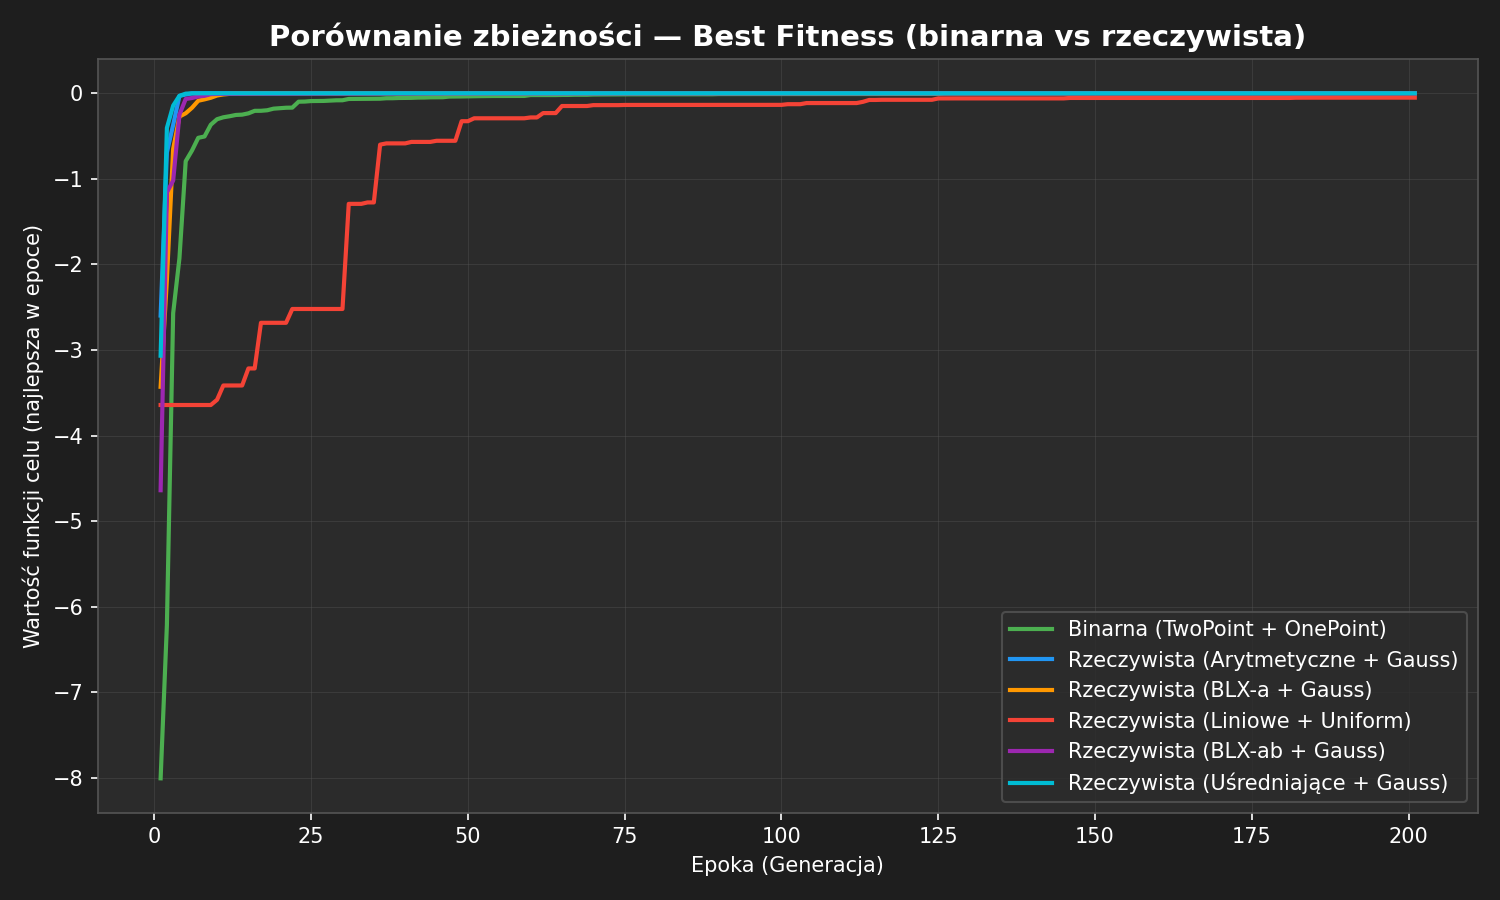
\includegraphics[width=0.9\textwidth]{img/p2_best_comparison.png}
    \caption{Zbieżność najlepszego osobnika w epoce (Wartość funkcji celu vs Iteracja)}
    \label{fig:best}
\end{figure}

Wykres najlepszego osobnika wykazuje szybką trajektorię odnajdywania bliskich rejonów minimum. Wyraźnie widać skokową redukcję wartości kosztu w pierwszych paru pokoleniach. Rzeczywista implementacja -- za sprawą np. równomiernej mutacji Gaussa czy też arytmetycznego krzyżowania zachowuje lepszą swobodę nawigacji niż skoki binarne. Reprezentacja liniowa sprawdziła się najgorzej na tym zbiorze w powiązaniu z dystrybucją jednostajną w mutacji.

\begin{figure}[H]
    \centering
    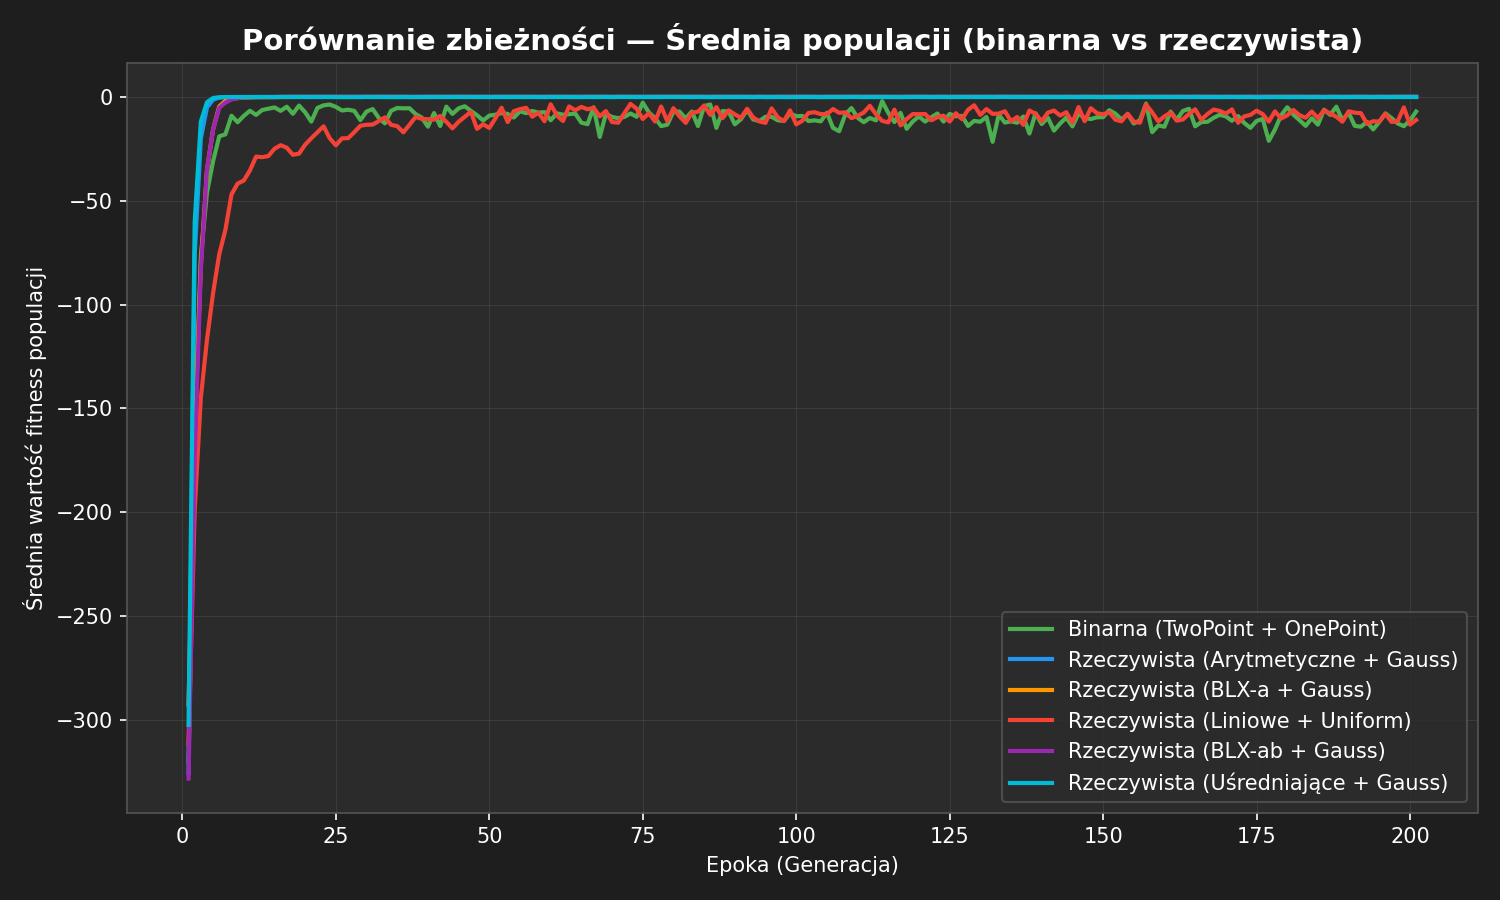
\includegraphics[width=0.9\textwidth]{img/p2_avg_comparison.png}
    \caption{Zależność średniej wartości fitness populacji od generacji}
    \label{fig:avg}
\end{figure}

Średnia wartość wskazuje również, w jak szybkim i zdecydowanym tempie warianty z mieszaniem typu BLX oraz z konwencjonalnym uśrednianiem (wraz z mutacją rozkładem Normalnym) dążą i stabilizują całą populację blisko punktu rozwiązania optymalnego. Oznacza to, że zróżnicowanie genetyczne wygasa po pewnym etapie silnej zbieżności i skupia stado bardzo blisko celu.

\begin{figure}[H]
    \centering
    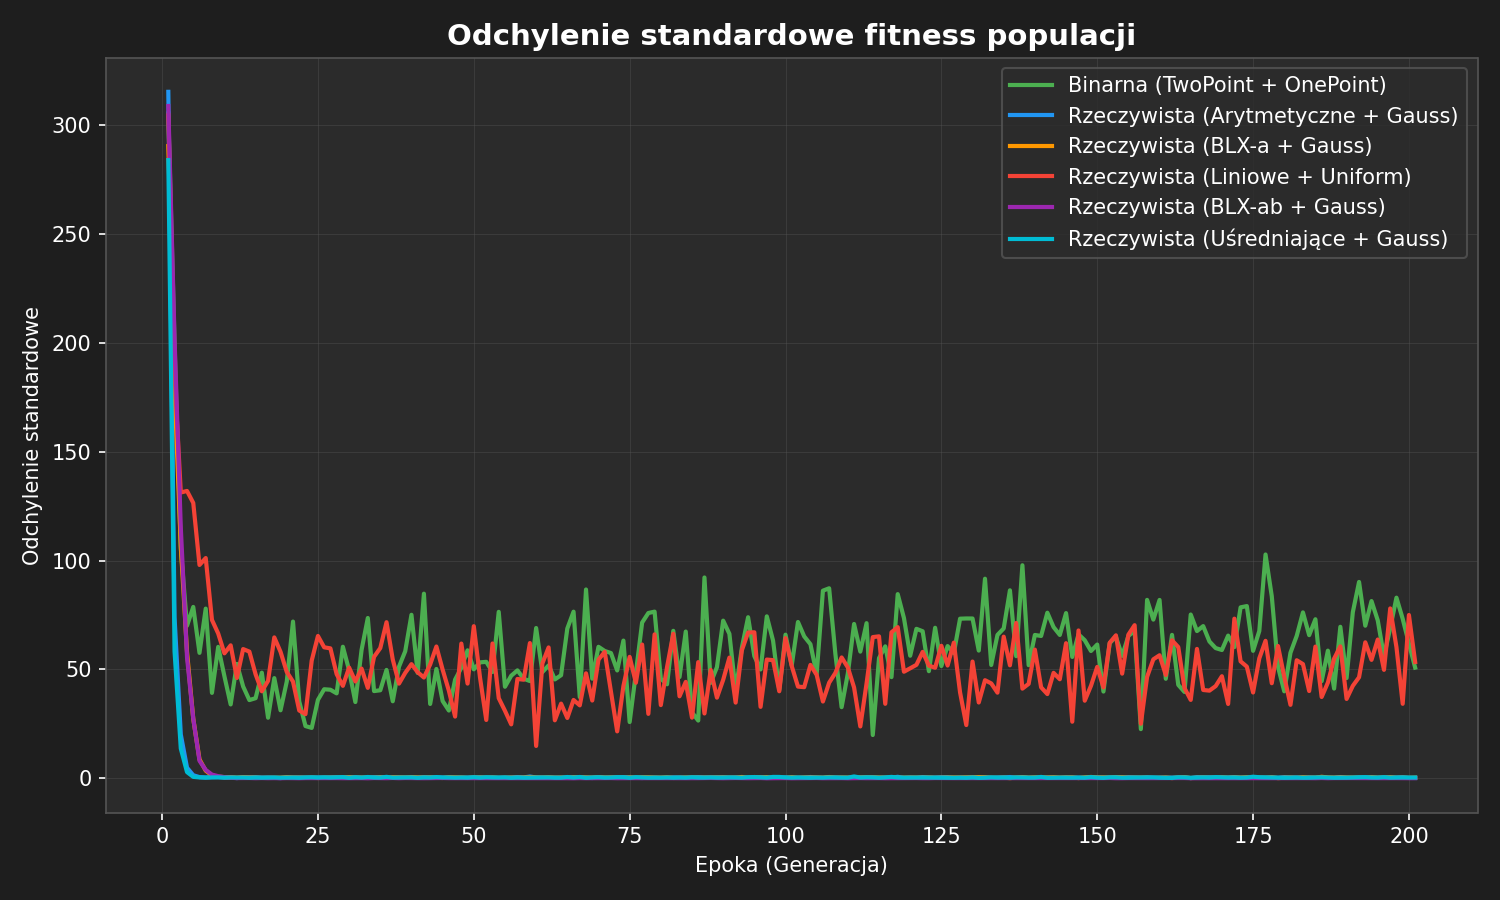
\includegraphics[width=0.9\textwidth]{img/p2_std_comparison.png}
    \caption{Przebieg odchylenia standardowego populacji podczas procesu optymalizacyjnego}
    \label{fig:std}
\end{figure}

Wykres \textbf{odchylenia standardowego} (\ref{fig:std}) potwierdza tę tezę, dobitnie sygnalizując stopniowe zacieśnianie osobnika wokół strefy sukcesu -- w późniejszych etapach wektory chromosomów dla wszystkich metod grawitują wokół $0$ (co sygnalizuje wysoką jednolitość i potencjalnie zatrzymanie ewolucji wskutek odnalezienia rozwiązania). Ciekawym jest zachowanie metody uśredniającej krzyżowanie z Gaussem, która ma duży rozstrzał w pierwszej generacji, by później dramatycznie zacisnąć wynik.

\section{Podsumowanie}
Modyfikacja architektury algorytmu z wariantu klasycznego na operujący w przestrzeni wielowymiarowych liczb rzeczywistych była sukcesem. Uniknięto skomplikowanej procedury dekodowania bitów co odbiło się na mocnym cięciu czasów ewaluacji z rzędu $>0.9s$ do rzędów $<0.5s$ dla testowanych ustawień.
Nowo powołane moduły operatorów mutacji i krzyżowania zachowują polimorfizm względem szkieletu i otwierają drogę do stosowania algorytmu na szerokie spektrum problemów dziedziny Data Science.

\end{document}
